\setchapterpreamble[u]{\margintoc}
\chapter{Third Lecture}
\labch{lec3}

% Will contain only signal flow graphs, system stability & singularities are shifted to lec 4 ... 

\section{Signal Flow Graphs}
\labsec{sec3.1}

\begin{figure}[h]
	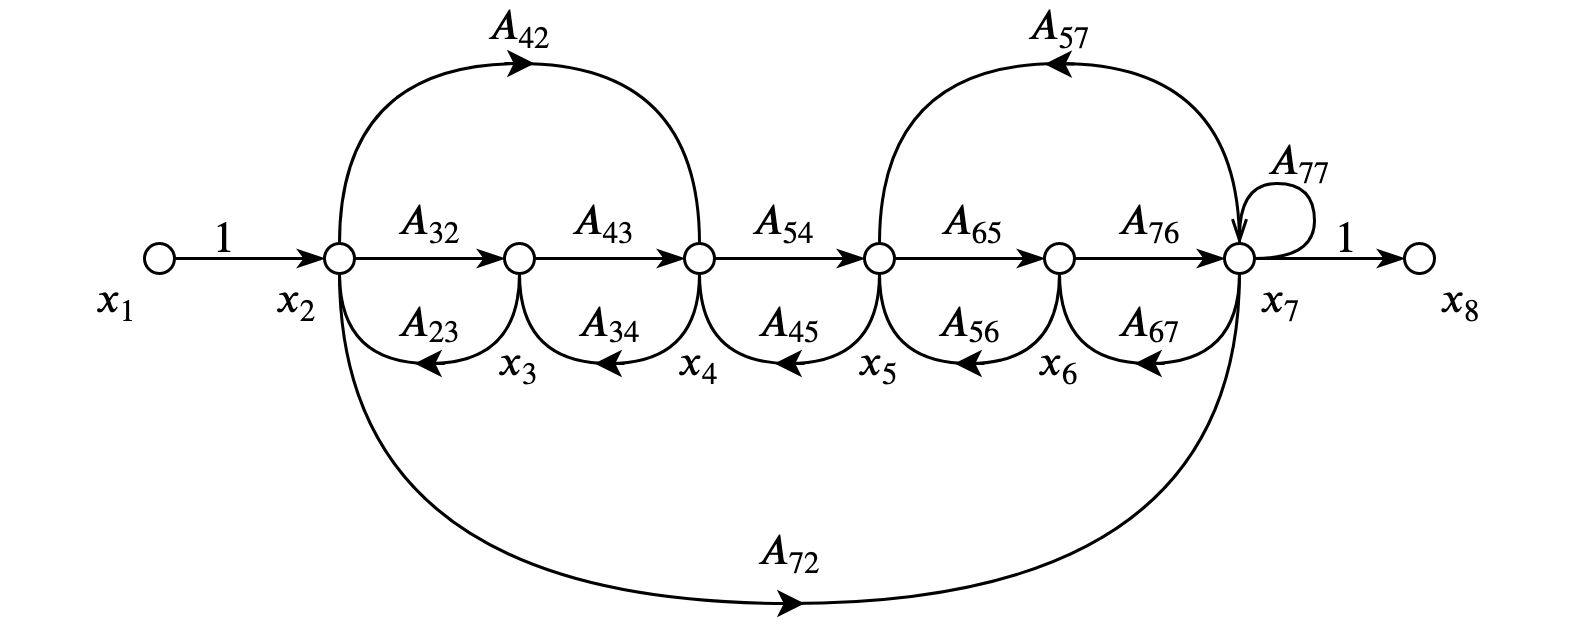
\includegraphics{lec3/Signal Flow}
	\caption{Signal flow general graph.}
\end{figure}

\subsection[Nodes]{Nodes\linkT{Reference: Feedback control system analysis and synthesis}}

\begin{description}
	\item[Source Nodes]  Represent independent variables and have only outgoing branches. ($x_1$)
	\item[Sink Nodes]  Represent dependent variables and have only incoming branches. ($x_8$)
	\item[Mixed Nodes]  Have both incoming and outgoing branches. ($x_2 \to x_7$)
\end{description}

\subsection[Paths]{Paths\linkS{http://imtiazhussainkalwar.weebly.com/feedback-control-systems-modeling-and-analysis.html}}

% [+0.42cm] is needed to allign with graphs that is not in margin, so -0.42 is good to allign with text.
% 0.4233401538135892 cm = 12 pt

\begin{description}
	\item[Forward Path]  From the input node to the output node.
		\begin{marginfigure}[-0.4233401538135892cm]
			\includegraphics{lec3/Forwards}
		\end{marginfigure}
	\vspace{2.7 cm}
	
	\item[Feedback loop]  Originates and terminates on the same node.
		\begin{marginfigure}[+0.4233401538135892cm]
			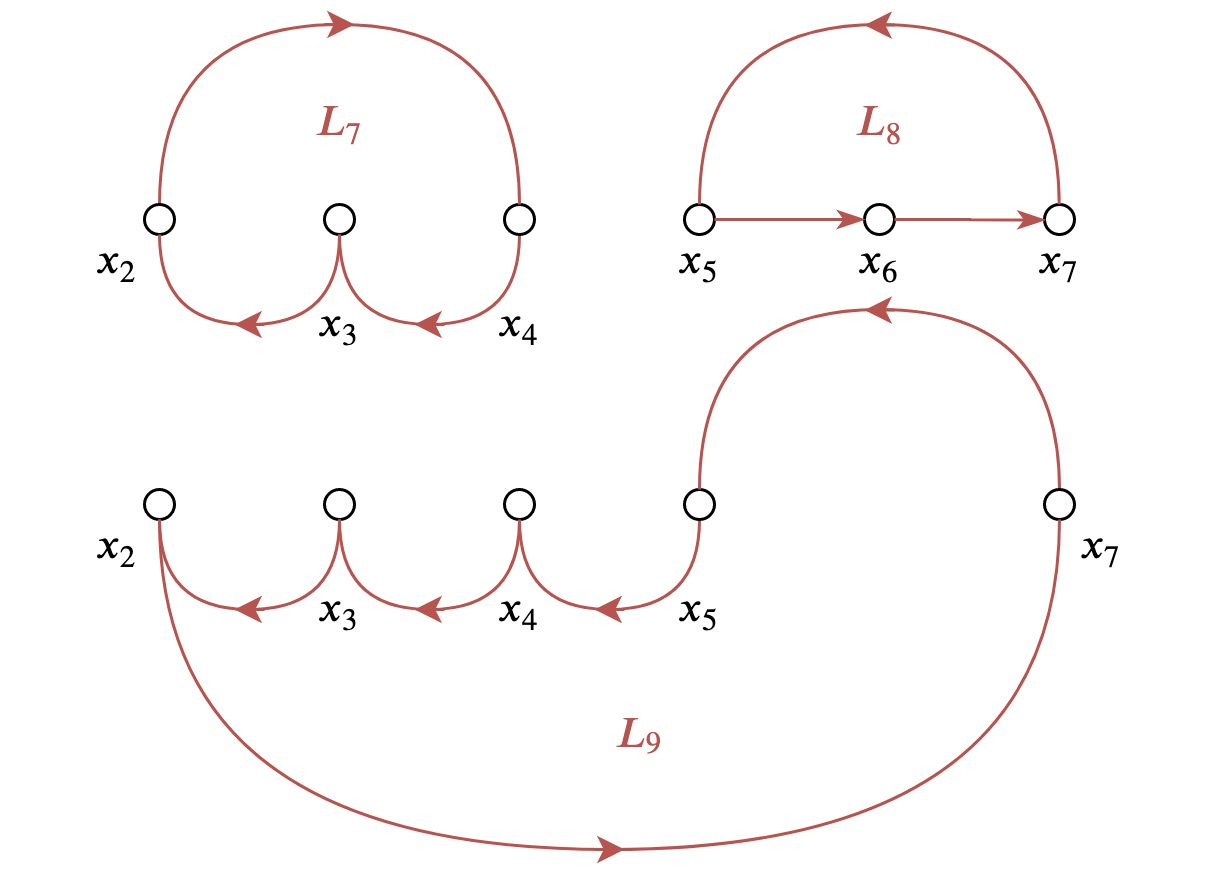
\includegraphics{lec3/Feedbacks - 2} 
		\end{marginfigure}
		\begin{figure}[h]
			\raggedleft
			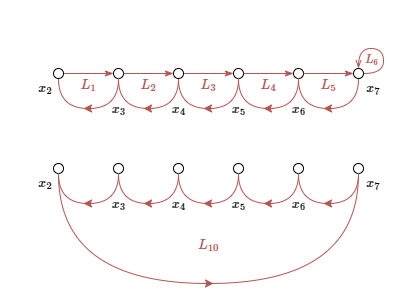
\includegraphics[width=\marginratio\textwidth]{lec3/Feedbacks - 1}
		\end{figure}
	
	\item[Self loop]  A feedback loop consisting of a single branch.
		\begin{figure}[h]
			\raggedleft
			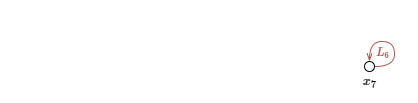
\includegraphics[width=\marginratio\textwidth]{lec3/A loop}
		\end{figure}
		
\end{description}

\subsection{Non-touching loops}

\raggedright
\begin{tabular}{r r r}
	\multicolumn{1}{l}{\textbf{Two at a time}} & \multicolumn{1}{l}{\ \ \ \ \ \textbf{Three at a time}} & \multicolumn{1}{l}{\ \ \ \ \ \textbf{Four at a time}} \\
	\raggedright
	\begin{tabular}{| c | c | c |}
	        \multicolumn{3}{c}{}\\[-1em]
	        $L_1L_3$ & $L_2L_4$ & $L_3L_6$ \\
	        $L_1L_4$ & $L_2L_5$ & $L_4L_6$ \\
	        $L_1L_5$ & $L_2L_6$ & $L_4L_7$ \\
	        $L_1L_6$ & $L_2L_8$ & $L_5L_7$ \\
	        $L_1L_8$ & $L_3L_5$ & $L_7L_8$ \\
	        \multicolumn{3}{c}{}\\[-1em]
	\end{tabular}&
	\raggedright
	\begin{tabular}{|c|}
	        \multicolumn{1}{c}{}\\[-1em]
	        $L_1L_3L_5$ \\
			$L_1L_3L_6$ \\
			$L_1L_4L_6$ \\
			$L_2L_4L_6$ \\
			$ $ \\
	        \multicolumn{1}{c}{}\\[-1em]
	\end{tabular}&\ldots\\
\end{tabular}

\subsection{Gain}
	
\begin{description}
	\item[Path Gain]  Product of branch gains encountered in a path. ($P_3:\ A_{72}$)
	\item[Loop Gain]  Product of the branch gains of the loop. ($L_3:\ A_{54}A_{45}$)
\end{description}

\section[Block to Flow-graph]{Block Diagram to Signal Flow Graph\linkS{https://www.tutorialspoint.com/control_systems/control_systems_signal_flow_graphs.htm}}
\labsec{sec3.3}

\begin{figure}[h]
			\centering
			\includegraphics[width=0.8\textwidth]{lec3/Motor Block Diagram}
			\caption{Motor block diagram.}
\end{figure}

\textbf{Step 1}\ \  Represent all the signals, variables,
summing points and take-off points of block diagram as nodes in signal flow graph.\\
\textbf{Step 2}\ \  Represent the blocks of block diagram as branches in signal flow graph.\\
\textbf{Step 3}\ \  Represent the transfer functions inside the blocks of block diagram as 
gains of the branches in signal flow graph.\sidenote[][]{Connect the nodes as per the block diagram.
If there is connection between two nodes (but there is no block in between),
then represent the gain of the branch as one.}\\[+2em]

\begin{figure}[h]
			\raggedleft
			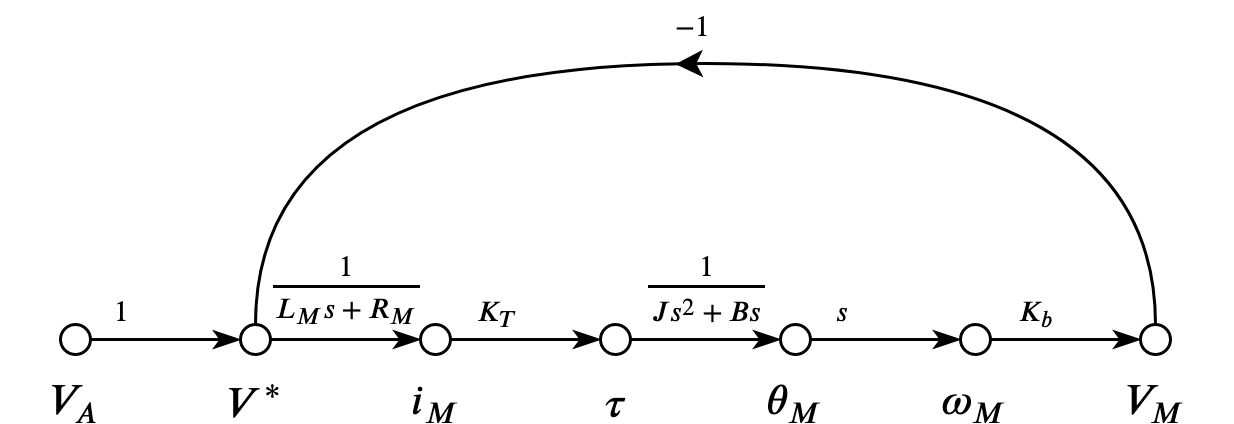
\includegraphics[width=0.7\textwidth]{lec3/Motor Flow Graph}
			\caption{Motor flow-graph diagram.}
\end{figure}

\section[Flow-graph Algebra]{Flow-graph Algebra\linkT{Reference: Feedback control system analysis and synthesis}}
\labsec{sec3.3}

\blindtext

\section{The Mason Rule}
\labsec{sec3.4}

\blindtext
